\documentclass[11pt, a4paper]{report}

\usepackage{graphicx}
\graphicspath{ {images/} }
\usepackage{caption}
\usepackage{subcaption}

\usepackage{hyperref}
\usepackage[xindy]{glossaries}
\makeglossaries
\makeindex

\usepackage[utf8]{inputenc}
\usepackage{csquotes}

\usepackage[square,sort,comma,numbers]{natbib}
\bibliographystyle{IEEEtran}

\usepackage{amsmath}
\newcommand\addtag{\refstepcounter{equation}\tag{\theequation}}
\usepackage{txfonts}

\usepackage{multirow}

\setlength{\parindent}{0ex}
\setlength{\parskip}{1ex}

%Rechtangle painting
\usepackage{tikz}
\usepackage[framemethod=tikz]{mdframed}

\mdfdefinestyle{mdthight}{
    linewidth=1pt,
    innerleftmargin=0bp,
    innerrightmargin=0bp,
    innertopmargin=0bp,
    innerbottommargin=0bp
}

\begin{document}

\title{
    
\includegraphics[width=1.75in]{fhnw_fhnw_logo_en.png} \\
    \vspace*{1in}
    \textbf{Report Street Networks}}
\author{
    Authors: \\
    Samuel Merki\\
    Janis Peyer\\
    \vspace*{0.4in} \\
    Coordinator: \\
    Prof. Dr. Stefan Arisona
    \vspace*{0.4in} \\
    Client: \\
    Chair of Information Architecture,
    ETH Zürich
    \vspace*{0.4in} \\
    Course of Studies: \\ Bachelor of Science in Computer Science
    \vspace*{0.4in} \\
    Institute of 4D Technologies \\
    \textbf{University of Applied Sciences and Arts  }\\
    Northwestern Switzerland FHNW
} \date{\today}
\maketitle
\setcounter{page}{1}

\tableofcontents

\begin{abstract}
    TODO: Text Here.
\end{abstract}

\chapter{Introduction}
To analyse and generate streets there are many approaches. Street networks can be described as grammars. 

The street networks can be divided into reasonable parts by clustering algorithms. 

The cluster can be evaluated by measurement methods provided by the architecture department of the ETH-Zurich. 
(Insert here how our work is used later!)
Genetic analysis of street network, separation, recombination.

TODO: Not completed!
\chapter{Street Network Grammars}
\section{Shape Grammar}
The main key of shape grammar is to generate paintings by a new defined grammar based on shapes, selection rules, painting rules and limiting shapes. Shape grammar is a language based on an alphabet of shapes and generated shapes \citep{shapeGrammars:1972}. 

A class of paintings defines the pair (S,M). S represents the shape specifications and M the material specifications. The shape specification contains a shape grammar, defining a language of two dimensional shapes, and a selection rule. M specifies a finite list of material specifications and one limiting shape on a canvas.

\subsection{Shape Grammar Definition}
\label{sec:Shape_Grammar_Definition}
Shape Grammar is defined over an alphabet of shapes and generated n-dimensional shapes \citep{shapeGrammars:1972}.
\begin{displayquote} 
    Definition. A shape grammar (SG) is a 4-tuple: $SG = (V_T, V_M, R, I)$ where
    \begin{enumerate}
        \item $V_T$ is a finite set of shapes.
        \item $V_M$ is a finite set of shapes such that $V_T $* $\cap$  $V_M = \emptyset$
        \item R is a finite set of ordered pairs (u,v) where:
        \begin{enumerate}
         \item u is a shape consisting of an element of $V_T $* combined with an element of $V_M$ \item v is a shape consisting of (A) the element of $V_T $* contained in u or (B) the element of $V_T $* contained in u combined with an element of $V_M$ or (C) the element of $V_T $* contained in u with an additional element of $V_T$* and an element of $V_M$.
        \end{enumerate}
        \item I is a shape consisting of elements of $V_T $* and $V_M$.
    \end{enumerate}
\end{displayquote}

\subsection{Selection Rules}
\label{sec:Shape_Grammar_Selection_Rules}
A painting is generated based on an undefined count of shape rules. This requires a mechanism to select a correct shape. The depth is defined by levels which are being assigned during generation based on their rules: \citep{shapeGrammars:1972}.
\begin{displayquote}
    \begin{enumerate}
        \item The terminals in the initial shape are assigned to level 0.
        \item If a shape rule is applied, and the highest level assigned to any part ot the terminal corresponding to the level side of the rule is N, then
        \begin{enumerate}
            \item if the rule is of type A, any part of the terminal enclosed by the marker in the left side of the rule is assigned to N.
            \item if the rule is of type B, any part of the terminal enclosed by the marker in the left side of the rule is assigned to N and any part of the terminal enclosed by the marker is assigned to N+1.
            \item if the rule is of type C, the terminal added is assigned to N+1.
        \end{enumerate}
        \item No other level assignments are made.
    \end{enumerate}
\end{displayquote}

\subsection{Painting Rules}
\label{sec:Shape_Grammar_Painting_Rules}
Painting rules describe witch shape should be painted inside of a defined area. Like in a Venn diagram the rules contain multiple levels 0 - n. By combining these levels the painting colour is described\citep{shapeGrammars:1972}.
\begin{displayquote}
    A painting rule has two sides separated by a double arrow ($\Rightarrow$). The left side of a painting rule defines a set using the sets determined by level assignment and the usual set operators, for example, union($\bigcap$), intersection ($\bigcup$), complementation($\sim$), and exclusive or ($\bigotimes$). The sets defined by the left side of the painting rules of M must partition the universal set. The right side of a painting rule is a rectangle painted in the manner the set defined by the left side of the rule is to be painted.
\end{displayquote}

\subsection{Limiting Shapes}
\label{sec:Shape_Grammar_Limiting_Shapes}
These shapes define a limiting area on the canvas, where shape painting is allowed. 
The area could have any form, but normally it is defined as a rectangle. Like a camera view the limiting shape defines the scale of a painting and its viewpoint. Therefore the initial/start shape could be outside of the limiting shape.

\subsection{Example\citep{shapeGrammars:1972}}
\subsubsection{Shape Grammar}
\begin{align}
\label{eq:Shape_Grammar}
SG1 &= <V_T, V_M, R, I>  \\
\label{eq:Shape_Grammar_VT}
V_T &= \{-\}  \\
\label{eq:Shape_Grammar_VM}
V_M &= \{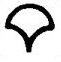
\includegraphics{sg_specification_VM.jpg} \}\ \\
\label{eq:Shape_Grammar_R}
R &= Rules\ [R]\ \ \ \ 
R1=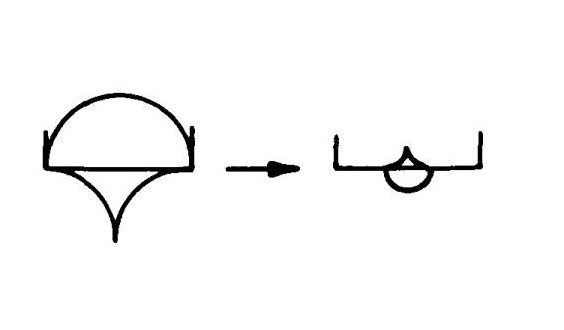
\includegraphics[width=2cm]{sg_specification_rule1.jpg}
R2=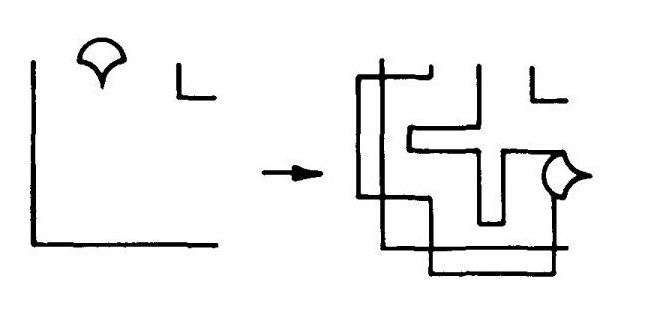
\includegraphics[width=2cm]{sg_specification_rule2.jpg}
R3=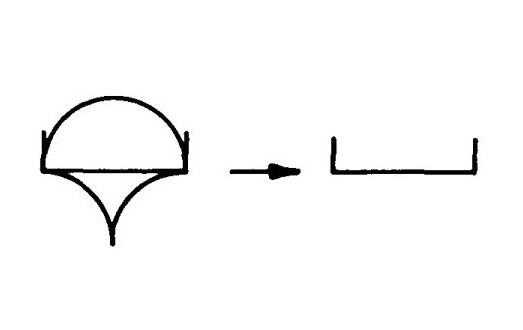
\includegraphics[width=2cm]{sg_specification_rule3.jpg}
\\
\label{eq:Shape_Grammar_I}
I &= Initial\ shape\ I\ \ 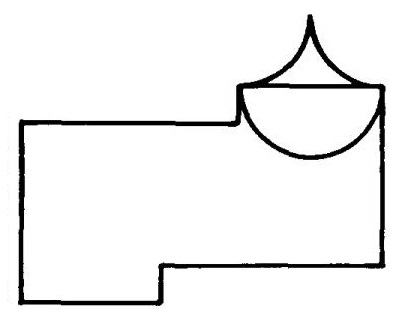
\includegraphics[width=1.5cm]{sg_specification_I.jpg}
\end{align}
\subsubsection{Selection Rule}
\begin{equation}
<0,2>
\end{equation}

\subsubsection{Painting Rules}
\begin{align}
    \label{fig:Shape Grammars/Shape Specification/Painting_Rule_1}
    L0\cap L1\cap L2 \Longrightarrow  
    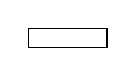
\begin{tikzpicture}
        \filldraw[fill=black!00!white, draw=black] (0,0) rectangle (1,0.25);
    \end{tikzpicture} \\
    \label{fig:Shape Grammars/Shape Specification/Painting_Rule_2}
    (L0\cap L1\cap \sim L2)\cup (L0\cap \sim L1\cap L2)\cup (\sim L0\cap L1 \cap L2) \Longrightarrow  
    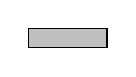
\begin{tikzpicture}
        \filldraw[fill=black!25!white, draw=black] (0,0) rectangle (1,0.25);
    \end{tikzpicture} \\
    \label{fig:Shape Grammars/Shape Specification/Painting_Rule_3}
    (L0\cap \sim L1\cap \sim L2)\cup (\sim L0\cap L1\cap \sim l2)\cup (\sim L0\cap \sim L1 \cap L2) \Longrightarrow  
    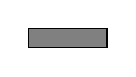
\begin{tikzpicture}
        \filldraw[fill=black!50!white, draw=black] (0,0) rectangle (1,0.25);
    \end{tikzpicture} \\
    \label{fig:Shape Grammars/Shape Specification/Painting_Rule_4}
    \sim (L0\cup L1\cup L2)  \Longrightarrow  
    
\begin{tikzpicture}
        \filldraw[fill=black!100!white, draw=black] (0,0) rectangle (1,0.25);
    \end{tikzpicture}
\end{align}
\subsubsection{Limiting Shape}
\begin{figure}[!h]
    \centering
    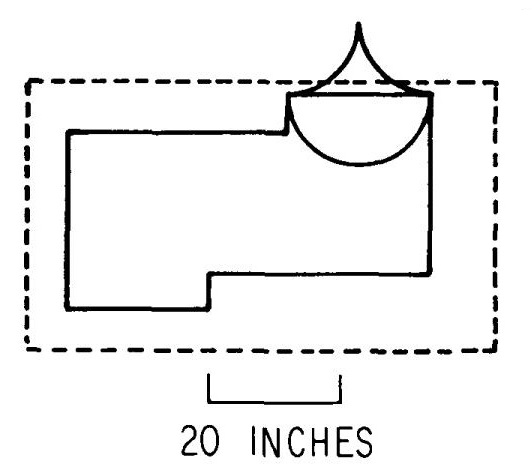
\includegraphics[width=2cm]{sg_specification_Limiting_shape.jpg}
    \caption{ Limiting shape I \citep{shapeGrammars:1972}}\label{fig:Shape Grammars/Shape Specification/Limiting_Shape}
\end{figure}
\pagebreak
\subsubsection{Generated}
The following image \ref{fig:Shape Grammars/Example} shows the generated painting with the relevant steps. The levels are generated as described above \ref{sec:Shape_Grammar_Selection_Rules} 
\newline
Level 0: Steps 0 to 2,\newline Level 1: Steps 3 and 4,\newline Level 2: Steps 18 and 19
\begin{figure}[!h]
    \centering
    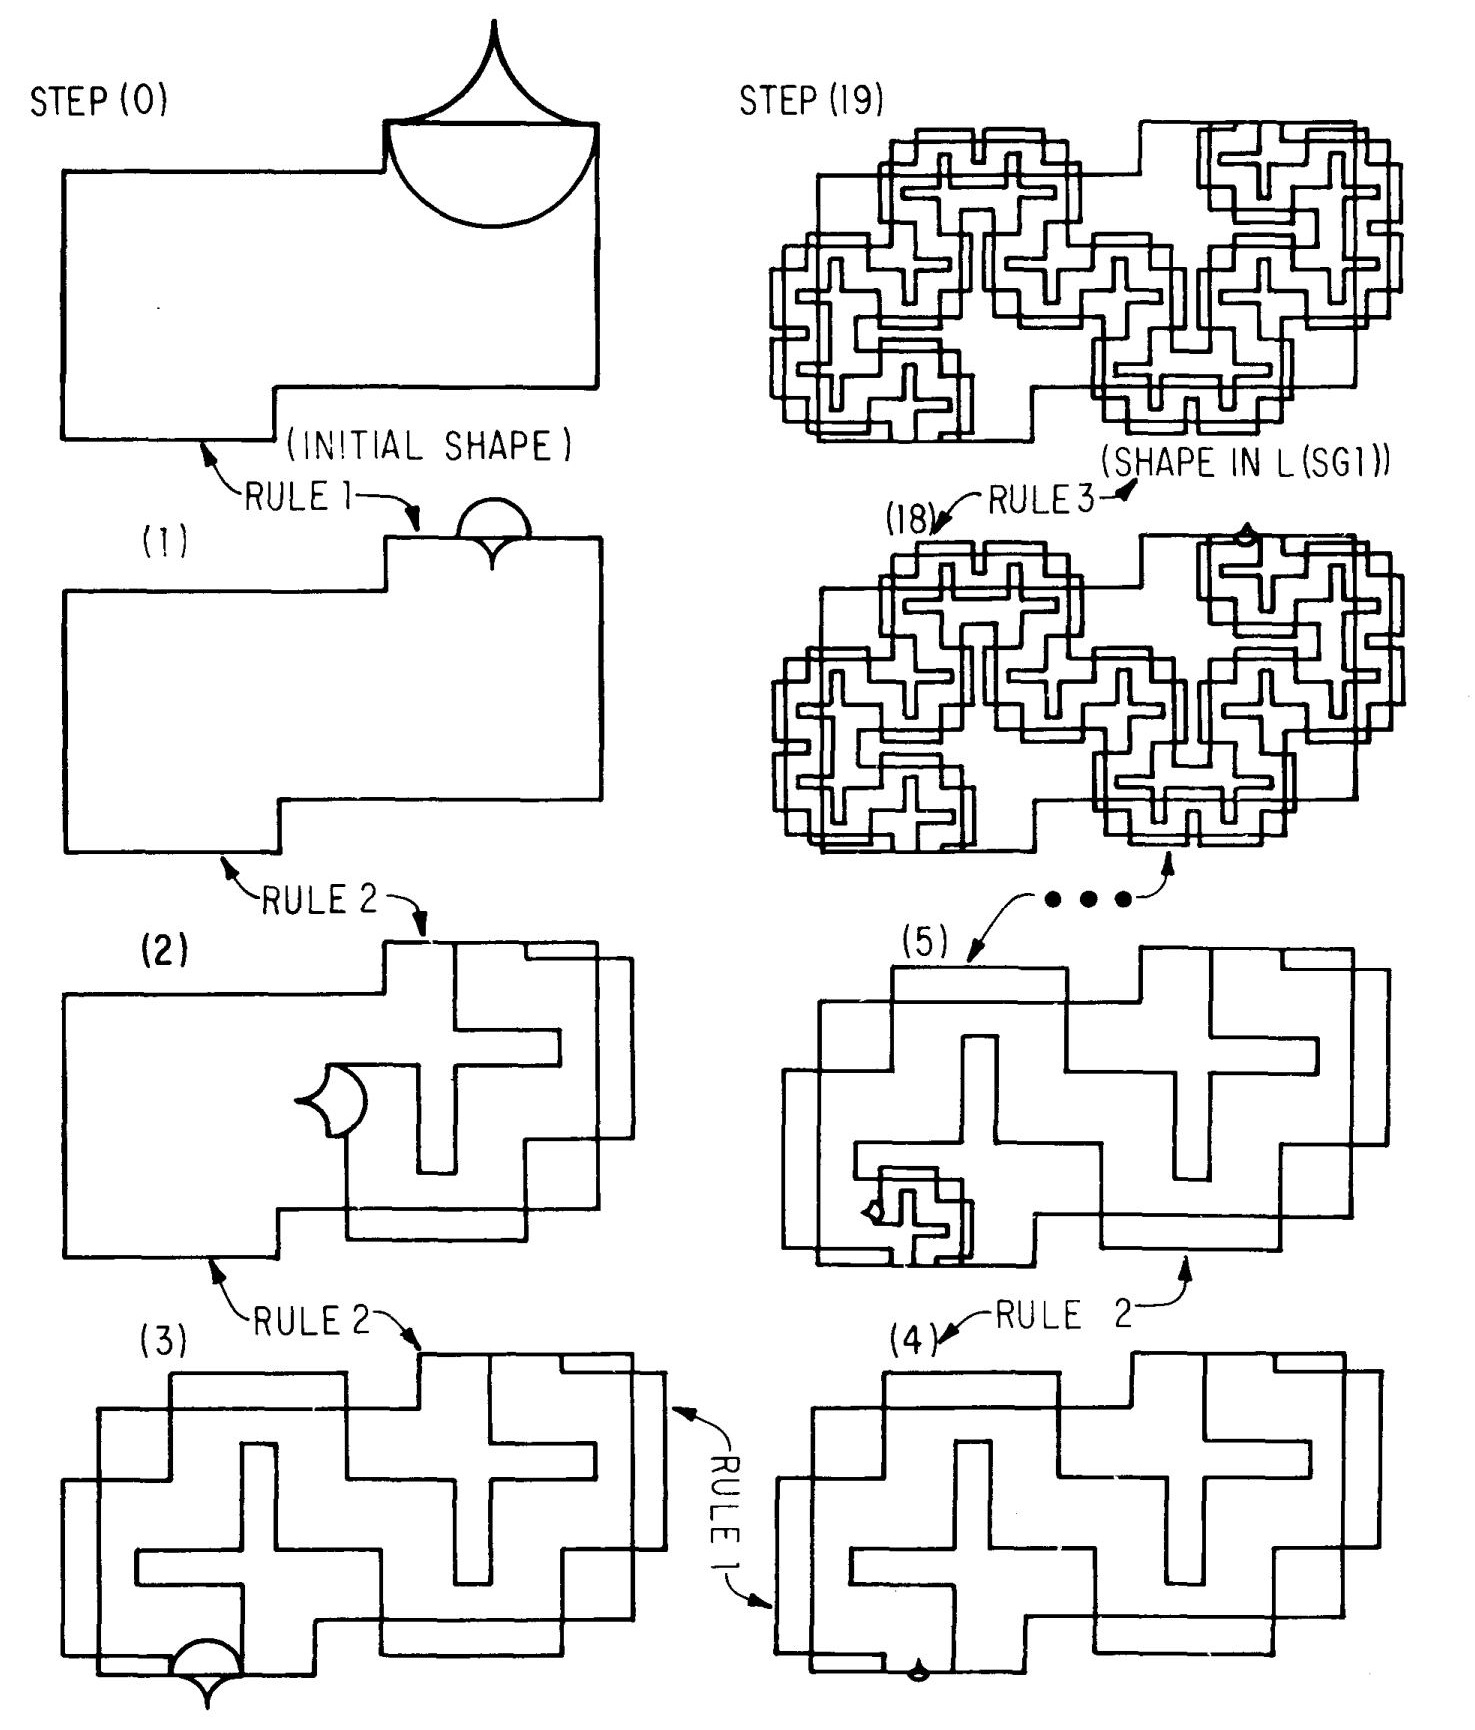
\includegraphics{sg_example.jpg}
    \caption{ Generated Painting\citep{shapeGrammars:1972}}\label{fig:Shape Grammars/Example}
\end{figure}

\pagebreak
\subsection{Street Generation}
In the following section we debate the usefulness of generating street networks by shape grammar. 
\paragraph{Features}
    \begin{itemize}
        \item Can describe and generate veneer in high details.
        \item With R-Shapes windows and high detail 3D-Models can be generated easily.
    \end{itemize}

\paragraph{Problems}
    \begin{itemize}
        \item The given methods generate monotonous streets in most cases. 
        \item A huge number of R-Shapes is required to generate a useful street network.
        \item Areas with different characteristics (historic district, rectangular raster like New York or radial to center like Paris) are difficult to generate.
        \item The R-Rules for the transitions between area characteristics should not repeat themselves and are for that reason difficult to build.
    \end{itemize}

\pagebreak
\section{L-Systems}
L-System is a well established modelling approach for the synthesis of realistic plant images. There are many papers describing L-Systems and how they are applied to generate plant life: "In these cases L-System productions capture the \textit{development} of plant components over time." \citep{PrusinkiewiczEtAl:2001} Productions are applied in parallel, so that all plant parts grow and age equally. The growth is stopped at a defined terminal age. This age is the number of iterations, where in each iteration productions are applied.

The context-free productions in \citep{PrusinkiewiczEtAl:2001} are defined using the following syntax.
\begin{equation} \label{eq:lsystem context free}
    pred : \{block1\}\ cond\ \{block2\} \leadsto succ
\end{equation}
The symbol \textit{pred} (predecessor) defines the module that will get replaced by the modules defined in \textit{succ} (successor). This replacement is only applied, if the (optional) condition is met. \textit{block1} and \textit{block2} are C statement blocks, of which the first block is executed before and the second after the condition is evaluated. \citep{PrusinkiewiczEtAl:2001} gives the following example.
\begin{equation} \label{eq:lsystem example 1}
    A(x) : \{y = x + 2;\}\ y \geq 5\ \{z = y / 3;\}\ \leadsto B(z)C(z + 1)
\end{equation}
If this example production was applied to the module $A(4)$, it would result in the modules $B(2)C(3)$.

The cpfg language, described in \citep{PrusinkiewiczEtAl:2001}, also supports context-sensitive productions. The following listing defines the syntax of such a production.
\begin{equation} \label{eq:lsystem context sensitive}
    lcont < pred > rcont : \{block1\}\ cond\ \{block2\} \leadsto succ
\end{equation}
\textit{lcont} (left context) and \textit{rcont} (right context) each define a list of modules that have to precede or respectively follow the \textit{pred} (module being replaced). Context modules are limited to query symbols, which are explained later on. \citep{PrusinkiewiczEtAl:2001} gives the following example.
\begin{equation} \label{eq:lsystem example 2}
    A(x) < B(y) > C(z) : x + z > 0 \leadsto M(y / 2)N(y / 2)
\end{equation}
If the example of listing \ref{eq:lsystem example 2} was applied to the module composition $A(2)B(4)C(0)$, it would result in the modules $A(2)M(2)N(2)C(0)$.

A way to generate images with L-Systems is to use a LOGO-style turtle as a graphical model. Certain modules of the L-System are interpreted as commands to this turtle.

\pagebreak
\section{Space Syntax}
The grammar Space Syntax was first introduced in 1976 by B. Hiller, A. Leaman, P. Stansall and M. Bedford in the paper "Space syntax" \citep{spaceSyntax:1976}. The grammar is based on a morphic language and describes methods to analyse and generate urban areas and buildings.
The language consists of a surface (carrier space) and an ongoing production process of new and different neighbouring parts. Extended Syntax is used to describe special area patterns like ring spaces and block spaces.

The grammar was later extended and integrated into Geographic Information System (GIS). This information system are used to plan and analyse the human interaction with the environment like pedestrian modelling or criminal mapping.
Bin Jiang and Christope Claramunt \citep{integrationSpaceSyntaxGIS:2002} showed the limitation of axial lined-based space syntax (\citep{integrationSpaceSyntaxGIS:2002} chapter: 2.2). They then created a graph representation (\citep{integrationSpaceSyntaxGIS:2002} chapter: 3) and showed that it was at least equivalent to the predefined syntax created by B. Hiller et al.\citep{spaceSyntax:1976}.

Many projects have been developed based on the space syntax graph representation. 

\pagebreak
\chapter{Clustering Algorithms}
In the application CPlan the street network is generated as a graph as described in \ref{CPlan}. To separate and select areas with specific characteristics the networks have been analysed by machine learning clustering algorithms. In this section the different clustering algorithms are analysed and the generated results produced by our implementations in CPlan are compared.
\section{K-Means}
\subsection{Description}
The K-Means algorithm detects the clusters / partitions by measuring the euclidean distance between the cluster centroids and the position of the street junctions. The algorithm uses the following approach:

\begin{enumerate}
    \item A number of points are inserted into the graph and used as centroids.
    \item All graph points are assigned to their nearest centroids.
    \item The centroids are moved to the center of their assigned graph points.
    \item Until the maximum number of iterations is reached this process is repeated starting by loop item 2.
\end{enumerate}
Because the K-Means algorithm can find local minima, this process needs to be executed more than once. The result with the best found solution will be selected.

\subsection{Implementation}
The added implementation in CPlan\citep{cPlan:2015} is an optimised K-Means version based on the paper \textit{An Efficient k-Means Clustering Algorithm: Analysis and Implementation} \cite{kmeans:2002} with a runtime of $O(n\ insert\ here)$

\subsection{Speed Optimization}
The ETH-Zurich provided the following networks: Bad Berka (552 nodes, 626 edges), Weimar (2012 nodes, 2646 edges) and Zurich (27446 nodes, 35121 edges). The network Zurich with factor 13 more edges than Weimar resulted in long processing time. A speed improvement can be achieved by running the K-Means iterations in parallel. Every iteration can be executed free of side effects. The measurements and comparisons of the results are provided in the section Practical Task/Measurements \ref{sec:measurements};

\subsection{Result}
The implementation in CPlan \ref{CPlan} produced the following image \ref{fig:KmeansGenerated} based on the city of Weimar. All streets in one cluster are marked with the same colour, the transitions between clusters are marked black.
\begin{figure}[!h]
    \centering
    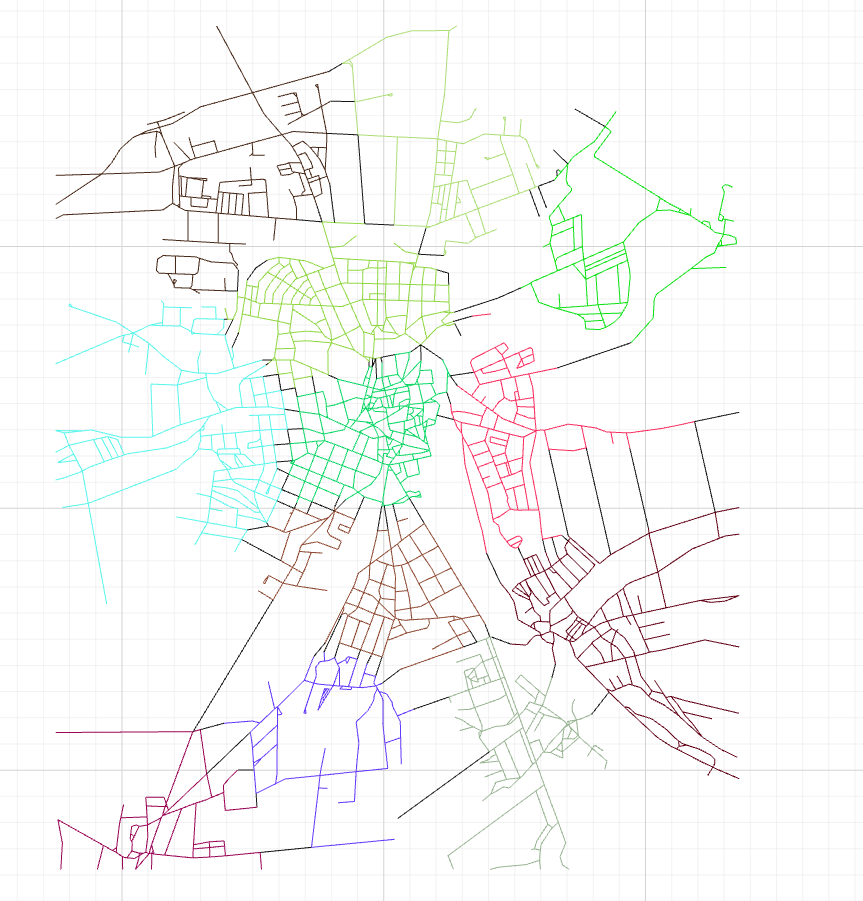
\includegraphics[width=\textwidth]{clusteranalysis_kmeans_result.png}
    \caption{K-Means cluster analysis of Weimar\label{fig:KmeansGenerated}}
\end{figure}

\subsection{Problem} \label{kmenasProblem}
The algorithm is based on the euclidean distance between cluster centroids and street junctions, the edge data (e.g. street length) is not used. As a result it leads to unexpected transitions between clusters. In the image \ref{fig:KmeansProblem} the result can be seen in the read circle where only one point is marked as outer cluster. The two black lines represent the cluster transitions.
\begin{figure}[!h]
    \centering
    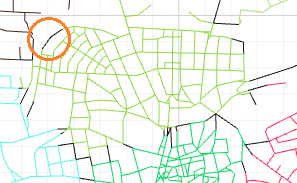
\includegraphics[width=0.6\textwidth]{clusteranalysis_kmeans_problem.png}
    \caption{Problem of K-Means clustering\label{fig:KmeansProblem}}
\end{figure}

\subsection{K-Means with Shortest Path}
To solve the problem of unexpected transitions between clusters the best result of the K-Means algorithm can be combined with the distance measurement of a shortest path algorithm (Dijkstra / FloydWarshall). These algorithms are used by hierarchical clustering \ref{hierarchicalClustering}. The edges are assigned by the edge data (e.g. street length) to the nearest cluster. Therefore the result is a connected graph. This means every vertex can be reached from every other vertex within a cluster. In the generated figure \ref{fig:Kmeansshortestp} the artefacts described in \ref{kmenasProblem} are removed.

Additional calculation time is needed for the shortest path algorithm. The differences can be compared in the section Practical Task/Measurements \ref{sec:measurements};

\begin{figure}[!h]
    \centering
    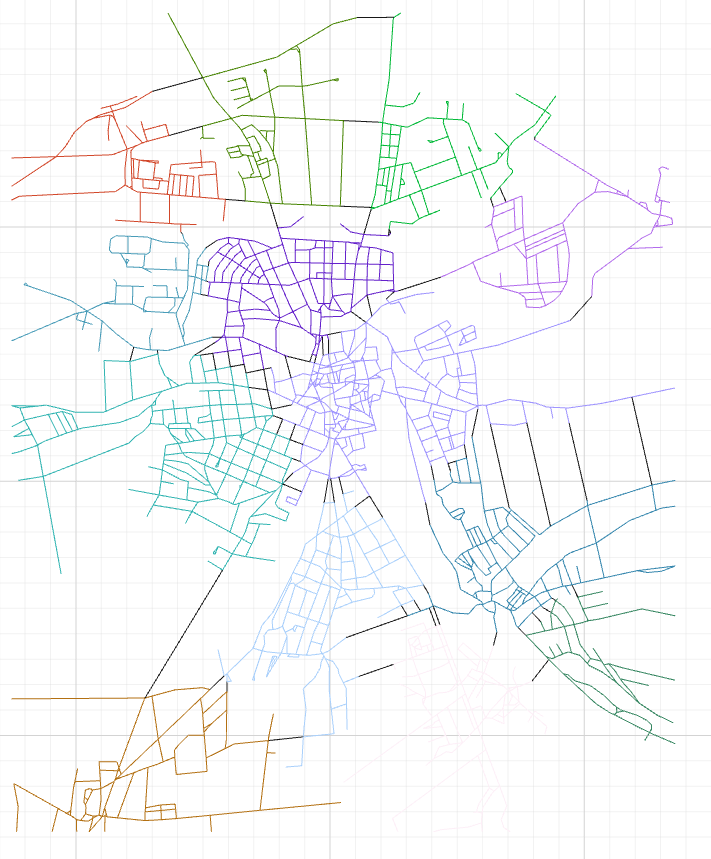
\includegraphics[width=0.9\textwidth]{clusteranalysis_kmeansExt_result.png}
    \caption{K-Means clustering with shortest path\label{fig:Kmeansshortestp}}
\end{figure}

\section{Hierarchical Clustering} \label{hierarchicalClustering}
\subsection{Introduction}
Hierarchical clustering, also known as connectivity based clustering, was the next applied approach. This area of algorithms clusters nodes together, which are near to each other. The advantage over K-Means is that graph distances can be used instead of the euclidean distance.

The result of a hierarchical clustering algorithm is a tree (or hierarchy), hence the name. This result can be used to create 1 to n clusters, where n is the number of input nodes.

\subsection{Strategy}
There are generally two main strategies for hierarchical clustering:

\begin{itemize}
    \item \textbf{Agglomerative}: Bottom up strategy. In the beginning each node is an own cluster. Clusters are combined until only a single cluster remains.
    \item \textbf{Divisive}: Top down strategy. All nodes are contained in one cluster at the start. This cluster is then divided into sub clusters.
\end{itemize}

The time complexity of the divisive strategy with $O(2^n)$ is too bad for the size of the street networks on which the algorithms have to run. The agglomerative strategy runs in $O(n^2 log(n))$ and in some special cases in $O(n^2)$ time complexity. The hierarchical clustering algorithms implemented for this thesis run in $O(n^2)$ time complexity. They are based on the paper "Optimal implementations of UPGMA and other common clustering algorithms" \cite{clustering:2007}.

\subsection{Reduction Formula}
The reduction formula is used to determine the distance between two clusters.
The following reduction formulae were implemented for this thesis:

\begin{itemize}
    \item \textbf{Single Linkage}
    \begin{multline}
    D_{Single-Linkage}(C_1, (C_2 \cup C_3)) \leftarrow \\
    min \{ D_{Single-Linkage}(C_1, C_2), D_{Single-Linkage}(C_1, C_3) \}
    \end{multline}
    \item \textbf{UPGMA}
    \begin{equation}
    \begin{split}
    D_{UPGMA}(C_1, (C_2 \cup C_3)) \leftarrow &\frac{|C_2|}{|C_2|+|C_3|}D_{UPGMA}(C_1, C_2)\ + \\ &\frac{|C_3|}{|C_2|+|C_3|}D_{UPGMA}(C_1, C_3)
    \end{split}
    \end{equation}
    \item \textbf{WPGMA}
    \begin{equation}
    D_{WPGMA}(C_1, (C_2 \cup C_3)) \leftarrow \frac{1}{2} (D_{WPGMA}(C_1, C_2) + D_{WPGMA}(C_1, C_3))
    \end{equation}
\end{itemize}

With clusters $C_1$, $C_2$ and $C_3$, which are sets of nodes and the distance function $d(i, j)$, which determines the distance between nodes $i$ and $j$.

For every of these reduction formulae the following holds:

\begin{equation}
\begin{split}
&\textrm{let }C_1, C_2\textrm{ be clusters}, i \in C_1, j \in C_2 \\
&\textrm{if }|C_1| = |C_2| = 1 \\
&\textrm{then }D(C_1, C_2) = d(i, j)
\end{split}
\end{equation}

For both the single linkage and the UPGMA reduction formula exists a dissimilarity function (\ref{eq:df_single_linkage} and \ref{eq:df_upgma}). These are alternative formulations of the reduction formulae which determine the distance by traversing all nodes of both clusters. The created cluster hierarchy is not used in these functions. For the WPGMA reduction formula no dissimilarity function exists, as shown in \cite{clustering:2007}.

\begin{equation} \label{eq:df_single_linkage}
D_{Single-Linkage}(C_1, C_2) = \min_{i\in{C1}, j\in{C2}}\{d(i, j)\}
\end{equation}
\begin{equation} \label{eq:df_upgma}
D_{UPGMA}(C_1, C_2) = \dfrac{1}{|C_1||C_2|} \sum_{i\in{C1}, j\in{C2}}{d(i, j)}
\end{equation}


\subsection{Single-Linkage Result}
The figure \ref{fig:SingleLinkage} shows the result of a hierarchical cluster analysis using the single linkage reduction formula. The used distance function $d(i, j)$ was the shortest distance from $i$ to $j$ in the street graph. As it is clearly visible when looking at the result, this way of cluster analysis is not creating the desired output. There is one huge cluster in the middle and many one-node clusters at the border of the city.

The problem is caused by the used reduction formula. Single linkage uses the distance between the closest nodes of the compared clusters. This leads to the creation of clusters, where all connecting roads are long. In a city, where there are multiple connections from one junction to another most of the time, this tends to create one-node clusters for nodes, which are connected to the city by a single long road.

\begin{figure}[!h]
    \centering
    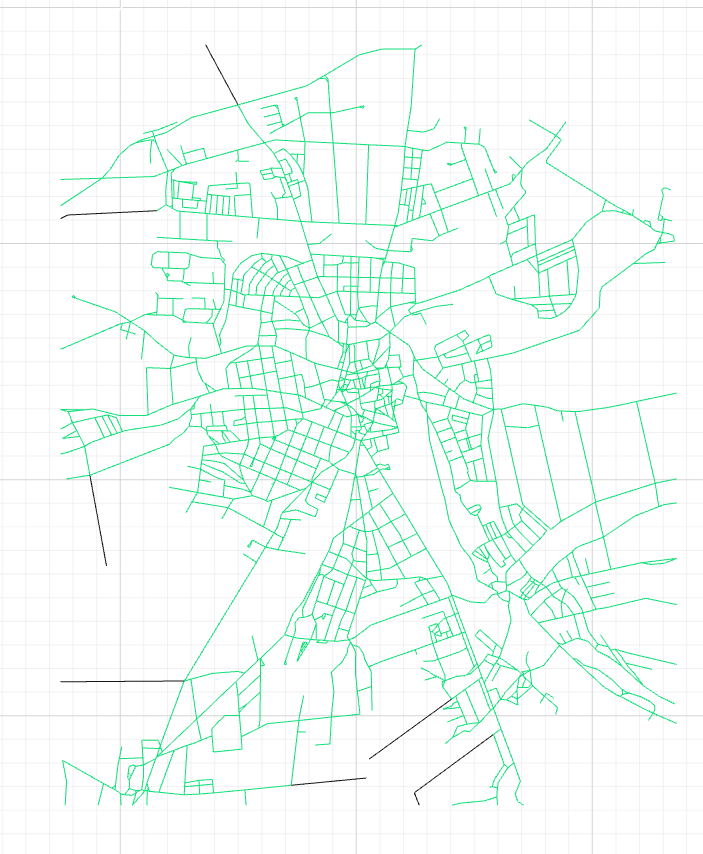
\includegraphics[width=\textwidth]{clusteranalysis_singlelinkage.png}
    \caption{Single-Linkage hierarchical cluster analysis of Weimar\label{fig:SingleLinkage}}
\end{figure}

\subsection{UPGMA and WPGMA Result}
\label{sec:UPGMAandWPGMA}
%TODO: Add figure
The figures xxx and xxx show the result of hierarchical cluster analysis using the UPGMA, or respectively the WPGMA reduction formula. The same distance function $d(i, j)$ as in the single linkage solution was used (shortest distance from $i$ to $j$ in the street graph).

\section{Cluster Rating}
\label{clusterRating}
To evaluate the generated clusters different measurement methods are necessary. Jun. Prof. Dr.  Reinhard König from the ETH Zurich provided the following parameters.
\newline
\begin{itemize}
    \item Geometry based measurements:
    \begin{itemize}
        \item Area based on the convex hull of the cluster area
        \item Total length of the streets
        \item Ratio between the area and total length
        \item Distribution variance of the street length
        \item Distribution variance of the street angles
        \item Ratio between street block size and surrounding circle area (minima, maxima, mean)
    \end{itemize}
    \item Centrality-based measurements normalized by the street count (minima, maxima, mean):
    \begin{itemize}
        \item In-Centrality (Integration)
        \item In-Betweenness-Centrality (Choice)
    \end{itemize}
\end{itemize}
The ratings can be calculated, compared and stored as JSON-File for each generated cluster in the CPlan \ref{CPlan} implementation.

Some initial measurements and comparisons are made in the cluster analysis chapter.

%TODO Images with examples with different clusters

\pagebreak
\chapter{CPlan}\label{CPlan}
CPlan is a tool written by the Department of Architecture of the ETH-Zurich. The goal of this application is to generate/grow street networks dynamically and extend these networks with buildings. 
\section{Improvements}
\begin{itemize}
    \item Some calls to the methods IEnumerable.ToArray() and IEnumerable.ToList() were removed. This method creates a new array / list and stores every item of the IEnumerable in this new collection. As a result the application had an extremely large footprint. To further reduce this overhead some methods were changed to take IEnumerable parameters instead of arrays.
    \item Certain graph and geometry extension methods were fixed. It would be good practice to create unit tests for such methods.
    \item matrix2D not clockwise? (TODO)
    \item Geometry2D not correct line intersection! (TODO)
\end{itemize}

\section{Genetic algorithms}
The ETH-Zurich already has genetic optimizations algorithms based on trees. Unfortunately they don't have a working solution to produce a tree from the existing graph. The new created tree generation produces a relative tree with absolute angles.

\pagebreak
\section{Normalising Street Networks}
While testing clustering algorithms on the street network of Zurich one rough spot of this network was found: Not all streets, which lead to a junction are connected to it. As shown in figure \ref{fig:zuerich_error} floating streets exist (highlighted in purple). No end of any of these highlighted streets is connected to the rest of the street network.

To handle those floating streets a network normalisation method was developed. The normalisation snaps (unites) all junctions and street end points, which are positioned close together, into one common junction. The result of this normalisation is shown in figure \ref{fig:zuerich_fixed}.

\begin{figure}
    \centering
    \begin{subfigure}[b]{0.8\textwidth}
        \begin{mdframed}[style=mdthight]
            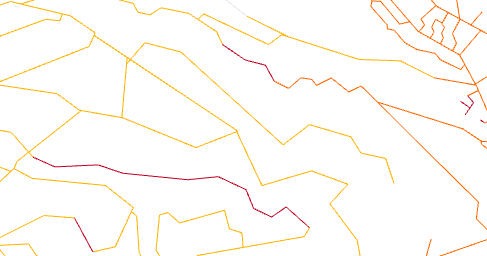
\includegraphics[width=\linewidth]{zuerich_street_error_cropped.png}
        \end{mdframed}
        \caption{Floating streets in the street network of Zurich}
        \label{fig:zuerich_error}
    \end{subfigure}
    \par\medskip
    \begin{subfigure}[b]{0.8\textwidth}
        \begin{mdframed}[style=mdthight]
            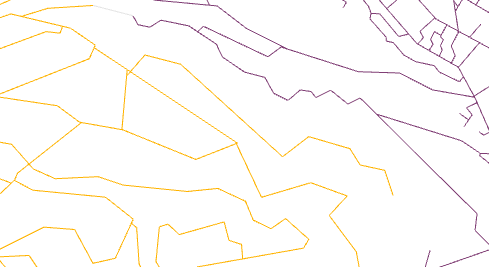
\includegraphics[width=\linewidth]{zuerich_street_fixed_cropped.png}
        \end{mdframed}
        \caption{Normalised street network of Zurich}
        \label{fig:zuerich_fixed}
    \end{subfigure}
    \caption{Street network of Zurich without (\ref{fig:zuerich_error}) and with (\ref{fig:zuerich_fixed}) normalisation}
\end{figure}

\section{Cluster colouring}
To visualize the clustering of a street network in this thesis, clusters are marked with different colours. This section describes the details of this cluster colouring.

The result of each clustering algorithm, which was implemented in this thesis, represents a cluster as set of vertices. Each of these vertices is a junction in the street network. The visualisation only draws streets but not the junctions, as the intersection of streets are intuitively seen as junctions. To colour the different clusters the following approach was taken:

\begin{itemize}
    \item Streets which connect two vertices that are part of the same cluster are coloured with that clusters colour.
    \item Streets which connect vertices of two distinct clusters are coloured grey.
\end{itemize}

There are papers which discuss how colours can be transformed to a perceptually uniform space, where the computation of $n$ colours with maximal distances (for the human eye) is possible \cite{colors:2006}.

In this thesis a more concise approach was taken: The papers of R. M. Boynton \cite{boynton:1989} and K. L. Kelly \cite{kelly:1965} define 11, respectively 22 colours, which are easy to distinguish by human eye. Those colours are displayed in figure \ref{fig:colours}.

Depending on the number of clusters one or the other of those colour sets (without black and white) were used. The colours were already sorted in a way that ensures the extraction of the first $n$ elements returns colours with maximal distance. If more than 20 clusters had to be coloured, the colours of Kelly were used multiple times.

\begin{figure}
    \centering
    \begin{subfigure}[b]{\textwidth}
        \begin{mdframed}[style=mdthight]
            
\includegraphics[width=\linewidth]{boynton_colours.png}
        \end{mdframed}
        \caption{Boynton colours}
        \label{fig:boynton_colours}
    \end{subfigure}
    \par\medskip
    \begin{subfigure}[b]{\textwidth}
        \begin{mdframed}[style=mdthight]
            
\includegraphics[width=\linewidth]{kelly_colours.png}
        \end{mdframed}
        \caption{Kelly colours}
        \label{fig:kelly_colurs}
    \end{subfigure}
    \caption{Colour palette of Boynton (\ref{fig:boynton_colours}) and Kelly (\ref{fig:kelly_colurs})}
    \label{fig:colours}
\end{figure}

\chapter{Measurements}
\label{sec:measurements}
In this following chapter the generated data with CPlan \ref{CPlan} is compared and analysed. 
\section{Speed Measurements}
\label{sec:measurements-speed}
TODO: Description of speed measurements here. 

TODO: Table of speed measurements here.

\section{Cluster Analysis}
\label{sec:measurements-cluster-analysis}
In this chapter the provided measurement methods \ref{clusterRating} are used to compare different districts/areas. The following images were generated with the cluster algorithm FastUPGMA \ref{sec:UPGMAandWPGMA} with \textit{Modified Output} and \textit{Number of Clusters} count 16. 

\subsection{Historic District}
\label{sec:historyDistinct}
This district is characterised by short streets with many connections. As a result the block areas are small and the block count per area is high. Additionally mean integration and mean choice values are high. This can be observed in the image \ref{fig:historic_district} and the measured data in table \ref{sec:ClusterAnalysisMeasurements} in column C1.
%TODO BILD

\begin{figure}
    \centering
    \begin{subfigure}[b]{0.6\textwidth}
        \begin{mdframed}[style=mdthight]
            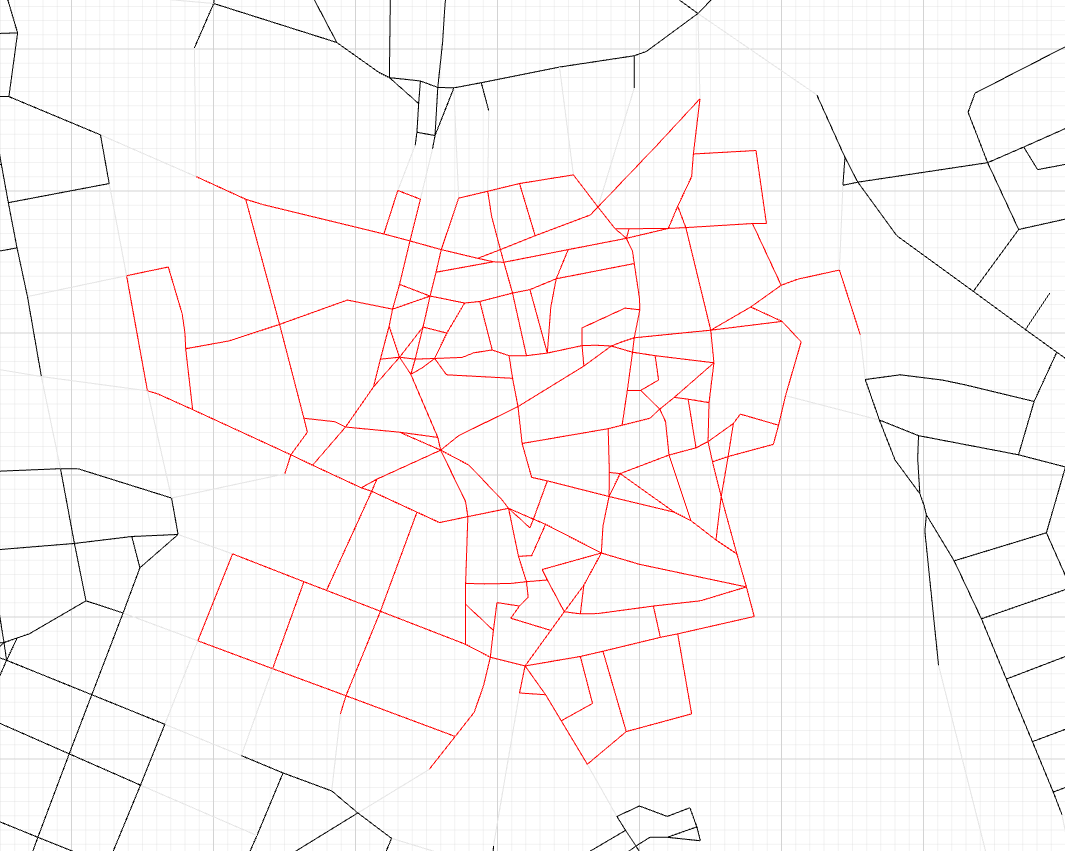
\includegraphics[width=\linewidth]{historic_district.png}
        \end{mdframed}
        \caption{Historic District of Weimar}
        \label{fig:historic_district}
    \end{subfigure}
    \par\medskip
    \begin{subfigure}[b]{0.6\textwidth}
        \begin{mdframed}[style=mdthight]
            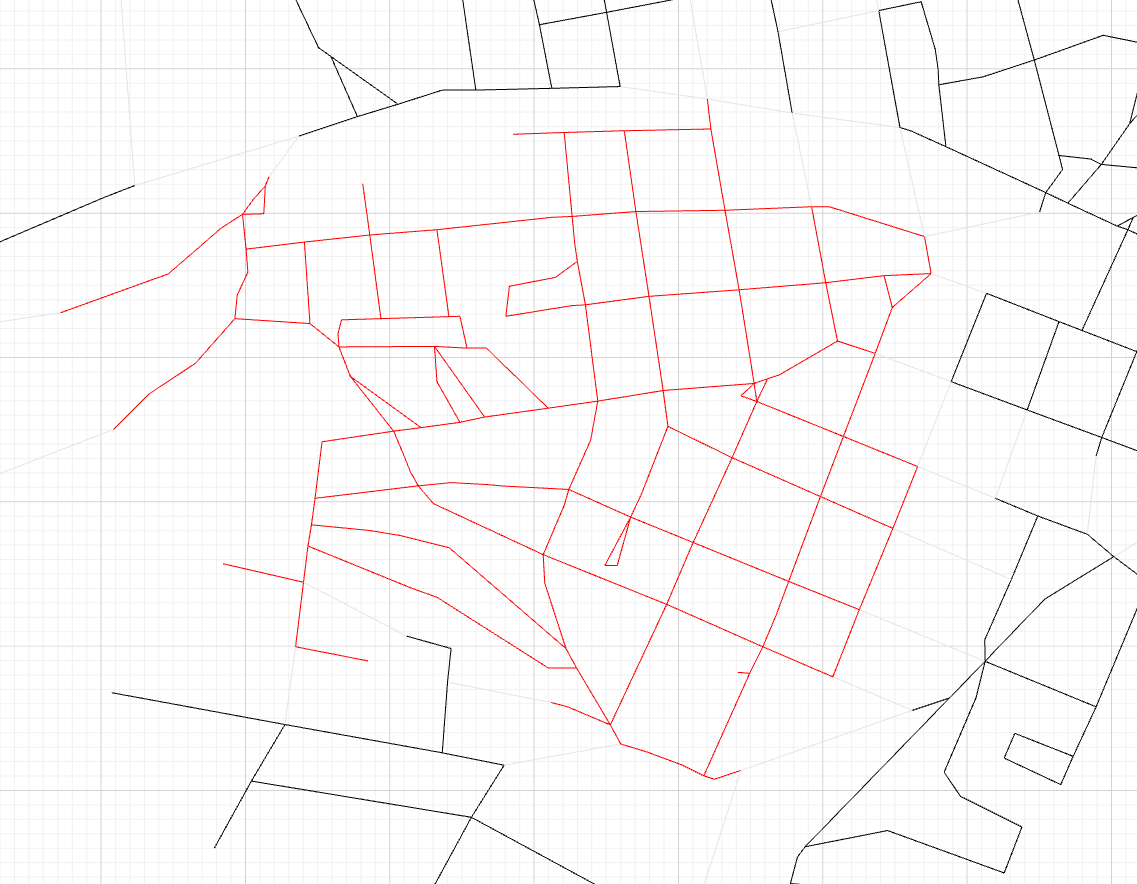
\includegraphics[width=\linewidth]{business_district.png}
        \end{mdframed}
        \caption{Business District of Weimar}
        \label{fig:business_district}
    \end{subfigure}
    \begin{subfigure}[b]{0.6\textwidth}
        \begin{mdframed}[style=mdthight]
            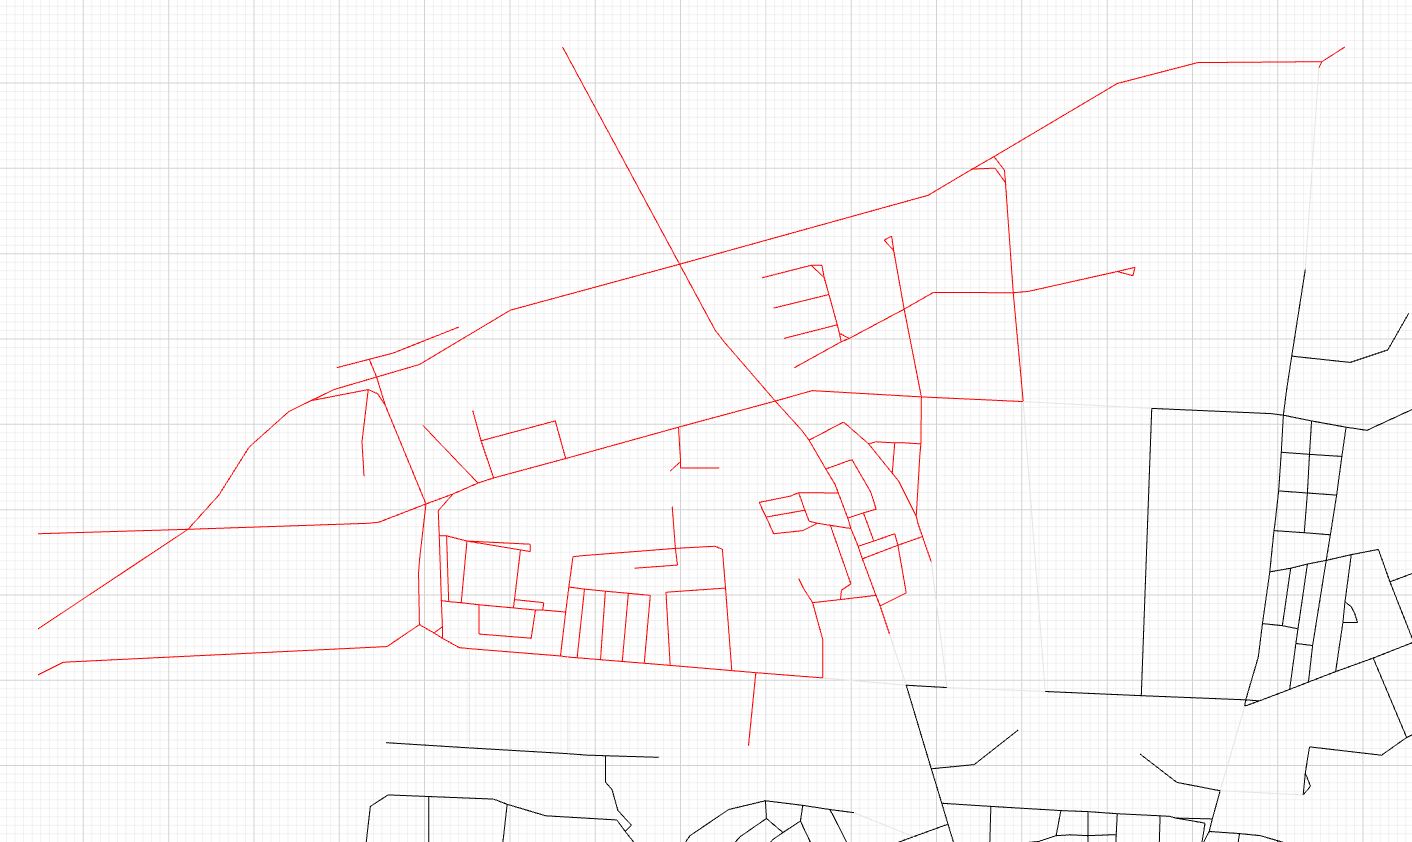
\includegraphics[width=\linewidth]{outskirts_district.png}
        \end{mdframed}
        \caption{Outskirts Area of Weimar}
        \label{fig:outskirts_district}
    \end{subfigure}
    \caption{Different areas of Weimar. Historic District (\ref{fig:historic_district}), Business District (\ref{fig:business_district}) and Outskirts Area (\ref{fig:outskirts_district})}
\end{figure}

\subsection{Business/Manhattan District}
\label{sec:businessDistinct}
If the block count and the connection count is high the given area is probably a business/Manhattan district. The street have a high mean connection count and the block area to circle area is high. The image REFTOIMG with the measured data in table \ref{sec:ClusterAnalysisMeasurements} in column C2, is an example area of this district/area type.

\subsection{Outskirts Area}
\label{sec:outskits}
These areas are characterized by extreme long streets and a low connection count as you can see in the example image REFTOIMG and the mesured data in table \ref{sec:ClusterAnalysisMeasurements} in column C3. The block count is compared with a business or historic district exceptional low.


\subsection{Measured Data}
\label{sec:ClusterAnalysisMeasurements}
The following table contains the parameters with additional descriptions. Extended information can be found below the table. Of every parameter the minimal (min), maximal (max), mean (average) and the median value can be calculated.

\begin{table}[h]
\begin{center}
    \begin{tabular}{ | l | l |} \hline 
        Parameter & Description \\ 
        \hline
        Total Area &  Area of the convex hull \\ \hline
        Total Length & Sum of the street length \\ \hline
        Density & Total Area divided to Total Length  \\ \hline
        
        Street Length Min/Max/Mean & Shortest/Longest/Average street length  \\ \hline
        Street Length Median & Middle value of the length dataset \\ \hline
        Street Length Variance & Sigma of the normal distribution curve of the variance \\ \hline
        
        Vertex Connections & Mean connected edges per vertex  \\ \hline
        
        Street Angle Min/Max/Mean & Smallest angle between two edges \\ \hline
        Street Angle Variance & Sigma of the normal distribution curve of the angles \\ \hline
        
        Block Count & Total number of blocks \\ \hline
        Block Area Min/Max/Mean & Shortest/Biggest/Average block area \\ \hline
        Block Area A/Ac Min/Max/Mean & Block area divided to a minimal circle around a block \\ \hline
        
        Integration Min/Max/Mean & Normalised In-Centrality \\ \hline
        Choice Min/Max/Mean & Normalised In-Betweenness-Centrality \\ \hline
    \end{tabular}
    \caption {Parameter with descriptions for table \ref{CPlan}}
\end{center}
\end{table}

\subsubsection{Block Area}
In the paper \textit{A typology of street patterns}\citep{blockArea:2014} the method is described how cities/areas can be classified and compared by analysing the block areas instead of the streets. First the block area is calculated and then the result is divided by the circumscribed circle area.

\subsubsection{Centrality}
The parameter \textit{Integration} describes the closeness centrality. This means the normed sum of the distances from all other vertex based on a shortest path algorithm is calculated. The vertex with the lowest value must be the most central.

With \textit{Choice} the betweenness centrality is described. The approach is to calculate the shortest path between every vertex. Every time a given vertex is visited the betweenness-centrality value of the vertex is raised by one. As a result the highest measured value indicates for a vertex to be in or near the centre of a graph.

\subsubsection{Variance}
The parameter variance describes the sigma of the normal curve of the distribution function.
First of all the measured data is round to fit into a distribution function \ref{eq:distribution_function}. Then the expected value \ref{eq:expected_value} and the variance \ref{eq:variance} is calculated. Finally the standard deviation (square root of V(x)) is computed \ref{eq:standard_deviation}.
\begin{align}
\label{eq:distribution_function} 
F(x) &= P(X \leq x) =  \sum_{t\in{X}, t\leq{x}}{f(t)} \\
\label{eq:expected_value} 
E(x) &= \int\limits_{-\infty}^\infty x * f(x)dx \\
\label{eq:variance} 
V(x) &= \int\limits_{-\infty}^\infty (x - E(X))^2 * f(x)dx \\
\label{eq:standard_deviation} 
\sigma(x) &= \sqrt{V(x)}
\end{align}

\begin{table}[h]
\begin{center}
\begin{tabular}{ |l|l|l|l|l|l| }
    \hline
    Parmater &  
    & C1 \ref{sec:historyDistinct} 
    & C2 \ref{sec:businessDistinct} 
    & C3 \ref{sec:outskits}
    & C4  \\ 
    \hline
    \multirow{4}{*}{Total} 
    & Area & 1838.05 & 1956.59 & & \\
    & Length & 806.92 & 643.50 & & \\
    & Density & 2.28 & 3.04 & & \\ 
    \hline
    \multirow{5}{*}{Street Length}
    & Min & 0.66 & 0.69 & & \\
    & Max & 9.13 & 10.68 & & \\
    & Mean & 2.72 & 3.85 &  & \\ 
    & Median & 2.30 & 3.65 & & \\ 
    & Variance & 1.70 & 2.19 & & \\ 
    \hline
    \multirow{1}{*}{Vertex} 
    & Connections & 3.04 & 2.84 & & \\
    \hline
    \multirow{5}{*}{Street Angle} 
    & Min & 0.00 & 0.00 & & \\
    & Max & 151.80 & 358.84 & & \\
    & Mean & 119.03 & 123.75 & & \\ 
    & Variance & 124.68 & 131.65 & & \\ 
    \hline
    \multirow{5}{*}{Block} 
    & Count & 55 & 35 & & \\
    & Area Min & 0.01 & 0.09 & & \\
    & Area Max & 31.75 & 42.29 & & \\
    & Area Mean & 6.54 & 13.65 & & \\ 
    & A/Ac Min & 0.01 & 0.01 & & \\
    & A/Ac Max & 0.54 & 0.55 & & \\
    & A/Ac Mean & 0.18 & 0.23 & & \\ 
    \hline
    \multirow{5}{*}{Integration} 
    & Min & 0.46 & 0.48 & & \\
    & Max & 0.57 & 0.75 & & \\
    & Mean & 0.49 & 0.59 & & \\ 
    \hline
    \multirow{5}{*}{Choice}
    & Min & 0.00 & 0.00 & & \\
    & Max & 1.00 & 0.67 & & \\
    & Mean & 0.10 & 0.05 & & \\ 
    \hline
\end{tabular}
\caption {Measured results from Cluster1 \ref{sec:historyDistinct}, Cluster2 \ref{sec:businessDistinct}, Cluster3 \ref{sec:outskits} and Cluster4}
\end{center}
\end{table}

\chapter{Possible Extensions}


\chapter{Conclusion}

\bibliography{quotations}
\appendix
\glsaddall
\printglossaries
\end{document}